
\documentclass{article}
\usepackage[utf8]{inputenc}
\usepackage[english]{babel}
\usepackage[]{amsthm} %lets us use \begin{proof}
\usepackage[]{amssymb} %gives us the character \varnothing

\usepackage{fullpage,amsmath,amssymb,graphics, graphicx,enumitem,ulem}

\title{Final Project}
\author{Jia Lin Yuan, }
\date\today
%This information doesn't actually show up on your document unless you use the maketitle command below

\begin{document}
\maketitle %This command prints the title based on information entered above

%Section and subsection automatically number unless you put the asterisk next to them.
\section*{}
%Basically, you type whatever text you want and use the $ sign to enter "math mode".
%For fancy calligraphy letters, use \mathcal{}
%Special characters are their own commands
\newpage
\subsection*{Problem 1}

\begin{enumerate}[label=\alph*]
    \item ${}$\\
    For distance by user we have: \\
    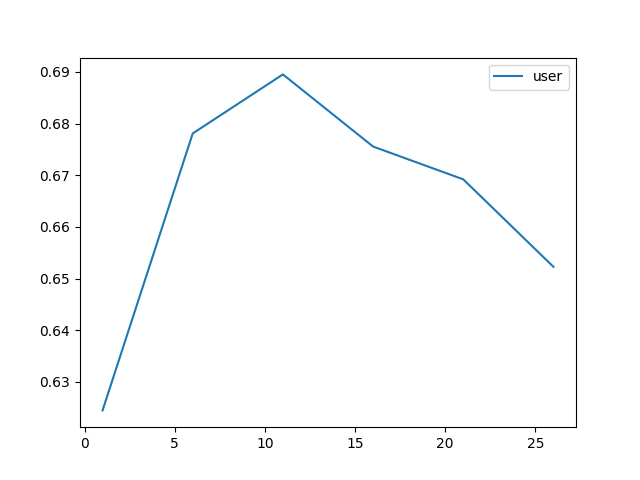
\includegraphics[scale=0.50]{../figs/knn_user.png}\\
    Validation Accuracy for k = 1: 0.6244707874682472\\
    Validation Accuracy for k = 6: 0.6780976573525261\\
    Validation Accuracy for k = 11: 0.6895286480383855\\
    Validation Accuracy for k = 16: 0.6755574372001129\\
    Validation Accuracy for k = 21: 0.6692068868190799\\
    Validation Accuracy for k = 26: 0.6522720858029918\\
    For distance by item we have: \\
    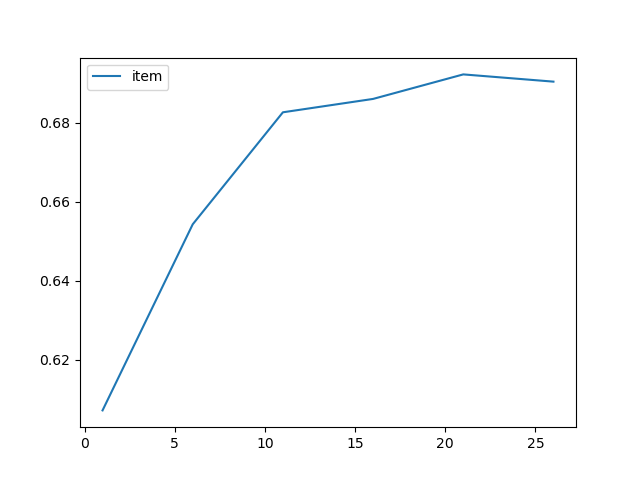
\includegraphics[scale=0.50]{../figs/knn_item.png}\\
    Validation Accuracy for k = 1: 0.607112616426757\\
    Validation Accuracy for k = 6: 0.6542478125882021\\
    Validation Accuracy for k = 11: 0.6826136042901496\\
    Validation Accuracy for k = 16: 0.6860005644933672\\
    Validation Accuracy for k = 21: 0.6922099915325995\\
    Validation Accuracy for k = 26: 0.69037538808919\\
    \item ${}$ \\
    We find that the best value for k for user-based collaborative filtering, k* is 11\\
    We find that the best value for k for item-based collaborative filtering, k* is 21\\
    
    \item (see code)
    \item Clearly item-based is better
    \item 1: Knn is slow. Even with only 542 items and 1774 users it takes a while to predict\\
    2: Using Euclidean distance, we consider distances in all dimension to be equal. For example if A and B's math skills are very different but english, physics, and other subjects are similar, the KNN will still predict A's math question similar to B's math questions (since skill in math is treated equally with other subjects).
\end{enumerate}

\newpage
\subsection*{Problem 2}
\begin{enumerate}[label=\alph*]
    \item 
\end{enumerate}
\end{document}